\chapter{Analyse}

Das vorherige Kapitel beschrieb die nötigen Technologien für die Realisierung und Ausführung einer Anwendung im Microservice-Architektur-Stil.
Dieses Kapitel beschäftigt sich nun mit der Analyse für die spätere Konzeptphase.

\section{Modernisierung der Infrastruktur}\label{moderninfra}
Dieser Abschnitt behandelt die aktuellen Bestrebungen der Krones AG hinsichtlich dem Aufbau einer modernen Infrastruktur in Produktionsanlagen. 
Zunächst wird der Proof of Concept, in dem die Umsetzbarkeit eines Kubernetes fähigen Konzept geprüft wurde behandelt. 
Anschließend werden Anwendungsmöglichkeiten im Bereich der Echtzeitkommunikation oder künstlichen Intelligenz untersucht. 

\subsection{Proof of Concept}
Die Krones AG entwickelt neue Konzepte, um Produktionsanlagen standortübergreifend zu modernisieren. 
In einem davon wurde ein \ac{poc} mit dem Software-Unternehmen SUSE durchgeführt, um die Umsetzbarkeit von Kubernetes-Technologien zu evaluieren. 
Diese beinhaltete die Aufrüstung einer Produktionsanlage mit Virtual-Edge-Devices, 
die über einen Hypervisor Typ 1 zwei Betriebssysteme gleichzeitig ausführen. Windows 10 Embedded, als \ac{hmi} und Linux SUSE Linux Enterprise Micro. 
Die Integration der Geräte ermöglicht die maschinennahe Nutzung von Echtzeitinformationen während des Betriebs und dienen als Fundament für den Aufbau einer wartungsfreien Infrastruktur.

\subsubsection{Kubernetes}
Die einzelnen Virtual-Edge-Devices sollen in Zukunft als Knotenpunkte für ein Kubernetes Cluster dienen. 
Dafür wird die für Edge-Szenarien entworfene Kubernetes-Distribution k3s installiert. 
Die Kubernetes-Cluster werden mit dem Orchestrierungstool Rancher verwaltet. 
Diese abstrahiert die Komplexität für den aktiven Betrieb von mehreren Clustern.


\subsection{Aufgabenstellung}
Im Zuge dessen wird die Umsetzbarkeit und Relevanz von Microservices auf der zukünftigen Produktionsanlage untersucht. 
Diese muss folgende Aufgabengebiete untersuchen.


\subsubsection{Bereitstellung}
Die Auslieferung und Entwicklung bestimmter Software soll zukünftig über Kundenrepositories erfolgen. 
Diese ermöglichen einen zentralen Ort für die kundenindividuelle Konfiguration der Anlagensoftware. 

\subsubsection{Hybrid Cloud}
Die Anwendung funktioniert in einem hybriden Cloud-Szenario mit unterschiedlichen Ressourcentypen. Kunden können sensible Daten in Ihrer eigenen
privaten Cloud oder einem lokalen Rechenzentrum speichern und gleichzeitig die
Vorteile von den erhöhten Rechenressourcen einer verwalteten Public Cloud nutzen.
Die flexible Wahl der Ressourcen ermöglicht kürzere Berechnungszeiten, ohne on-premise Hardware zu besitzen, die zur Auswertung und Evaluierung von Produktionsanlagen dienen.

\subsubsection{Echtzeitkommunikation}
Die Anwendung auf den Edge-Devices kommunizieren in Echtzeit miteinander. 
Und können die Informationen sinnvoll verarbeiten und persistent speichern.

\subsubsection{Künstliche Intelligenz}
Die Anwendung bringt einen Mehrwert im Bereich der künstlichen Intelligenz und nutzt die Infrastruktur zur Auswertung von Deep Learning Modellen. 

\section{Fachkonzept}
Im folgenden Abschnitt werden die Anforderungen und Anwendungsfälle für die spätere Konzeption der Microservice-Architektur erhoben.
Dafür wird ein zielorientierter Ansatz gewählt, der Anforderungen aus den Zielen einer Aufgabenstellung herleitet \cite[S.47]{Laplante}. 

\subsection{Anforderungserhebung}
Der vorherige Abschnitt \ref{moderninfra} beschreibt die Aufgabenstellungen, die mithilfe von Zielen erreicht werden können. 
Ziele sind erforderlich, um die zukünftigen Anforderungen der Software zu erarbeiten und werden in einer Anforderungstabelle wiedergeben (vgl. Tabelle~\ref{table:Anforderungstabelle}). 

\begin{table}[!htb]
\begin{center}

\begin{tabular}{|p{1cm}|p{6.8cm}|p{6.8cm}|l|l}
    \hline
    \textbf{Nr.} & \textbf{Ziele} & \textbf{Anforderungen} \\
    \hline
    \hypertarget{A01}{A01} 
    & Auf dem Kubernetes-Cluster laufen Anwendungen im Bereich der künstlichen Intelligenz.
    & Dienste sollen Funktionen der künstlichen Intelligenz ausführen können.
    \\
    \hline
    \hypertarget{A02}{A02}
    & Anwendungen auf einem Kubernetes-Cluster haben die Möglichkeit, Daten persistent zu speichern.
    & Dienste sollen über einen Speicher verfügen, der Daten persistent speichert.
    \\
    \hline
    \hypertarget{A03}{A03} 
    & Die einfache Auslieferung der Anwendung auf dem Kubernetes-Cluster ist möglich.
    & Die Dienste sollen über einen Auslieferungsmechanismus bereitgestellt werden.
    \\
    \hline
    \hypertarget{A04}{A04} 
    & Die Inbetriebnahme der Anwendung auf ein Kubernetes-Cluster ist vorkonfiguriert.
    & Dienste sollen vor der Inbetriebnahme vorkonfiguriert werden.
    \\
    \hline
    \hypertarget{A05}{A05} 
    & Die Anwendung funktioniert ohne die zusätzliche Installation von Abhängigkeiten auf dem Hostsystem.
    & Dienste sollen bei der Installation bereits über die nötigen Abhängigkeiten verfügen.
    \\
    \hline
    \hypertarget{A06}{A06} 
    & Die Anwendung kommuniziert in Echtzeit mit anderen Anwendungen auf dem Hostsystem.
    & Dienste sollen in Echtzeit miteinander kommunizieren.
    \\
    \hline
    \hypertarget{A07}{A07} 
    & Die Anwendung wurde vor der Inbetriebnahme auf dem Kubernetes-Cluster getestet.
    & Dienste sollen vor der Inbetriebnahme Tests durchlaufen.
    \\
    \hline
    \hypertarget{A08}{A08} 
    & Die Anwendung lässt sich für spezifische Hardware vorkonfigurieren. 
    & Dienste sollen bei Vorkonfiguration auf spezifischer Hardware laufen.
    \\
    \hline
\end{tabular}
\caption{Anforderungstabelle}
\label{table:Anforderungstabelle}
\end{center}
\end{table}

Die Tabelle gewährt einen groben Überblick der nötigen Systemanforderungen an die Mircoservice Architektur. 
Diese werden nun für das Konzept der Anwendung verwendet.
%Diese werden verfeinert und unterteilen sich im nächsten Abschnitt in Funktionale Anforderungen, also dem Grundverhalten, des Systems das der Nutzer erwartet und den nicht-Funktionale Anforderungen, den qualitativen oder leistungstechnischen Aspekten der Anwendung.



%\subsection{Funktionale Anforderungen}

%\textbf{Bereitstellung der Anwendung}: 
%Die Awendung muss sich auf einem Kubernetes Cluster, über eine Vorkonfiguration, bereitstellen lassen [\hyperlink{A01}{A01}]. 
%Bei der Bereitstellung muss die Anwendung, die nötigen Abhängigkeiten beeinhalten [\hyperlink{A05}{A05}]. 
%Zuletzt muss die Bereitstellung der Anwendung auf die Infrastruktur, Konfigurationen für spezifische Hardware enthalten [\hyperlink{A08}{A08}].
%Das 

%\textbf{Testprozess der Anwendung}: 
%Bevor die Anwendung verwendet wird, muss ein fester Testprozess die Funktionalität gewährleisten [\hyperlink{A07}{A07}].

%\textbf{Künstliche Intelligenz}: 
%Die Anwendung muss  [\hyperlink{A06}{A06}].



\subsection{Konzept}\label{Konzept}
Die prototypische Anwendung wird containerisert und über ein Registry verfügbar sein [\hyperlink{A03}{A03}] [\hyperlink{A05}{A05}]. 
Weiterhin muss die Anwendung unter der Berücksichtigung der Aspekte einer Microservice-Architektur, wie in Abschnitt \ref{Microservice} beschrieben, konzipiert und entwickelt werden. 
Die einzelnen Dienste der Anwendung müssen auf einem Kubernetes-fähigen Cluster ausgeliefert und in Betrieb genommen werden [\hyperlink{A04}{A04}].
Bevor die Anwendung verwendet wird, muss ein fester Testprozess die Funktionalität gewährleisten [\hyperlink{A07}{A07}].

Für die mögliche Auslieferung bei einem Kunden der Krones AG soll die Nutzung bereits vorhandener Hardware mit Grafikkarten möglich sein [\hyperlink{A08}{A08}]. 
Es ist vorgesehen, dass die Anwendung in einem hybriden Cloud-Szenario die vordefinierte Hardware nutzen kann. Folglich soll die Verwendung der Hardware zu einer verbesserten Leistungsauswertung von Modellen im Bereich der künstlichen Intelligenz führen. 
Arbeitslasten, wie dem Auswerten von Deep-Learning-Modellen wie im Falle der Linatronic AI \cite{linatronic}, sollen beispielhaft dargestellt werden [\hyperlink{A01}{A01}]. 
Dafür muss die Kommunikation von Diensten in Echtzeit stattfinden, um Informationen am Zielort schnell zu verarbeiten und eine nahtlose Verarbeitung großer Daten zu ermöglichen [\hyperlink{A06}{A06}].

\subsubsection{Anwendungsszenario}\label{Anwendungsszenario}

Der Schwerpunkt der zu entwickelnden Anwendung soll ein Dashboard mit Authentifizierungsmechanismus sein. 
Dieser soll Benutzern ermöglichen sich mit ihrem Passwort oder per Gesichtserkennung in ihr Profil einzuloggen. 
Die Daten sollen persistent gespeichert werden und können bei erneutem Aufruf der Website wieder verwendet werden [\hyperlink{A02}{A02}]. 

\subsection{Grobentwurf}

Auf der Grundlage von Abschnitt \ref{Konzept} werden die Grobentwürfe erstellt.
Die Konzeptentwürfe gliedern sich in zwei Teile, der Infrastruktur und der Anwendung.

\begin{figure}[!htb]
    \centering
    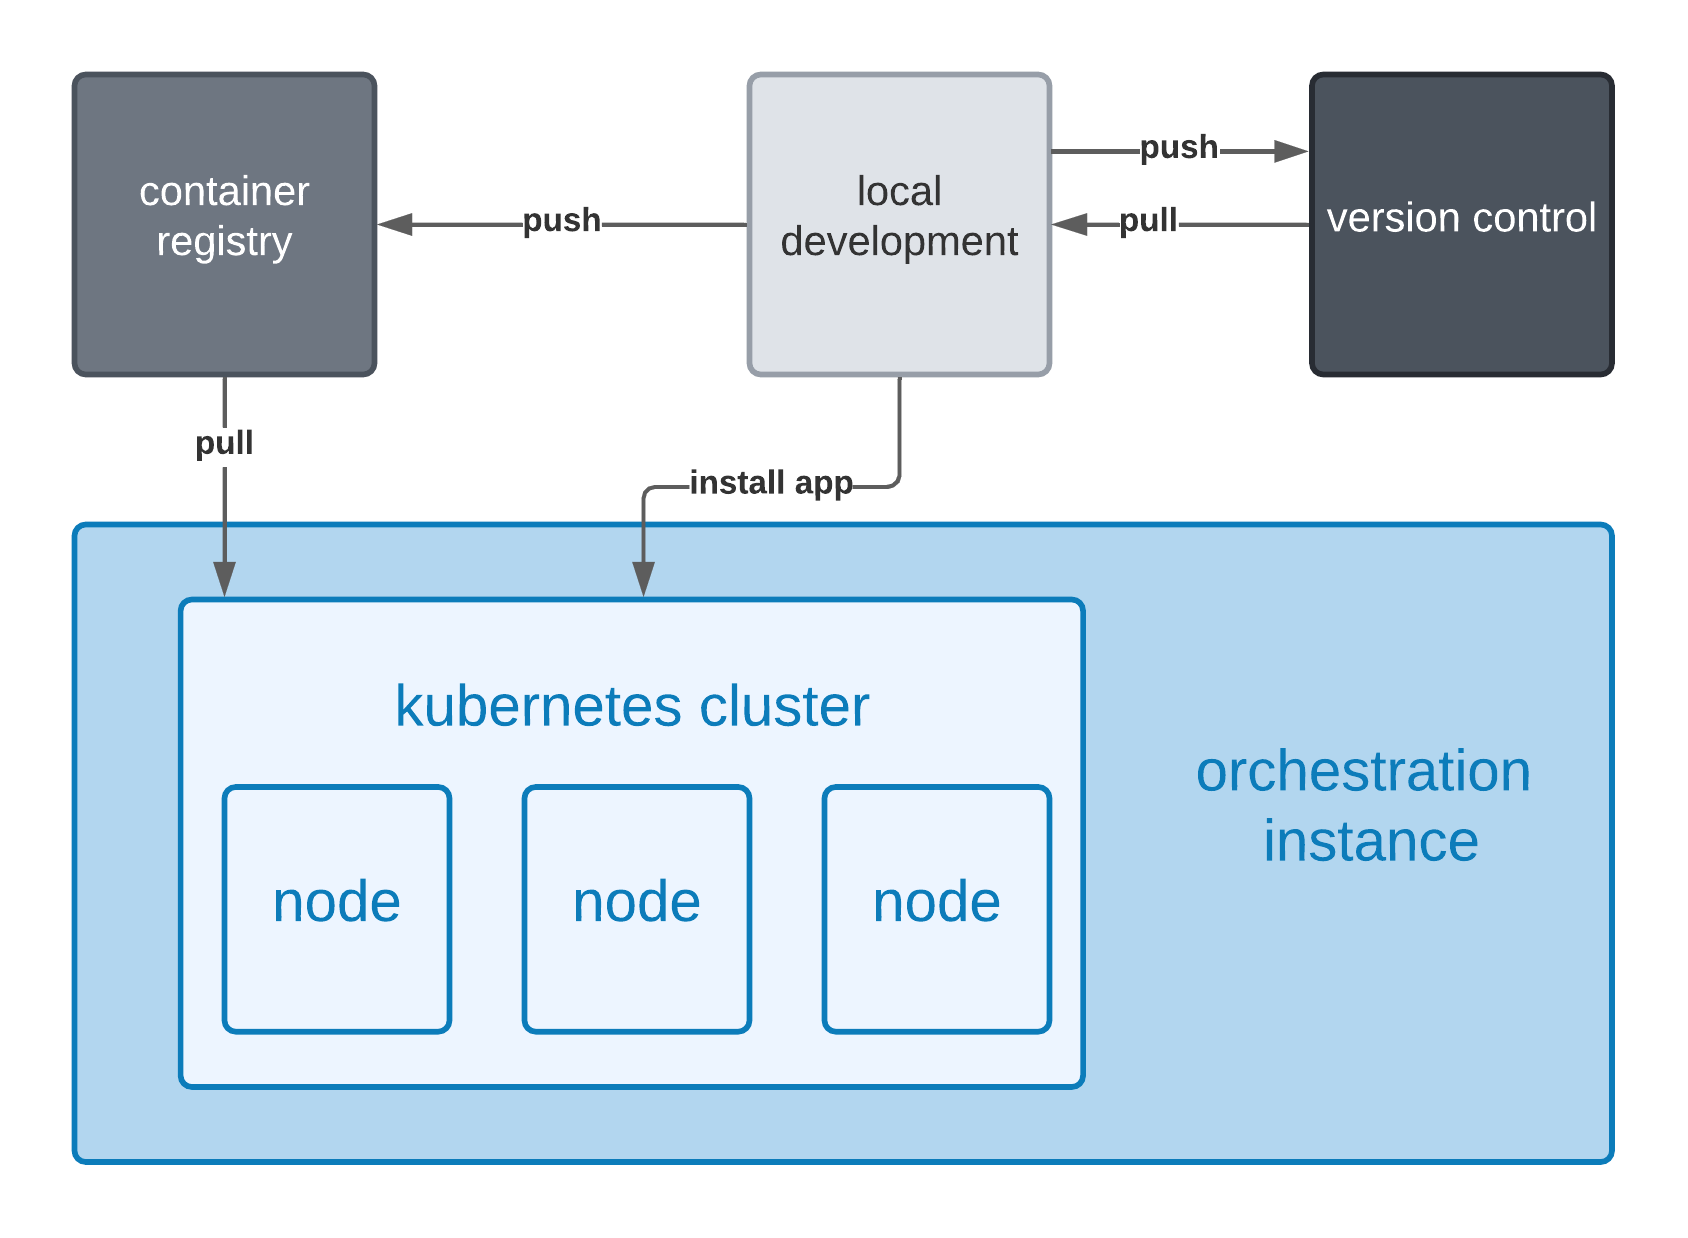
\includegraphics[width=0.8\columnwidth]{images/GrobentwurfInfrastruktur.png}
    \caption{Grobentwurf der Infrastruktur}
    \label{fig:GrobentwurfInfrastruktur}
  \end{figure}

\textbf{Lokale Entwicklungsumgebung}: Die Entwicklung der Anwendung verläuft lokal und wird durch ein Versionsverwaltungssystem verwaltet.
Ein Befehl an das Kubernetes-Cluster initialisiert die Auslieferung und Bereitstellung der einzelnen Dienste. 

\textbf{Image-Registry}: Für die Auslieferung und Bereitstellung von Containern wird ein Image-Registry verwendet.
Dienste erhalten seperate Images und können unabhängig abgerufen werden.

\textbf{Kubernetes-Cluster}: Das Kubernetes-Cluster wird von einer Orchestierungsinstanz verwaltet.
Das Abrufen der Dienste erfolgt über ein Image-Registry.

\begin{figure}[!htb]
    \centering
    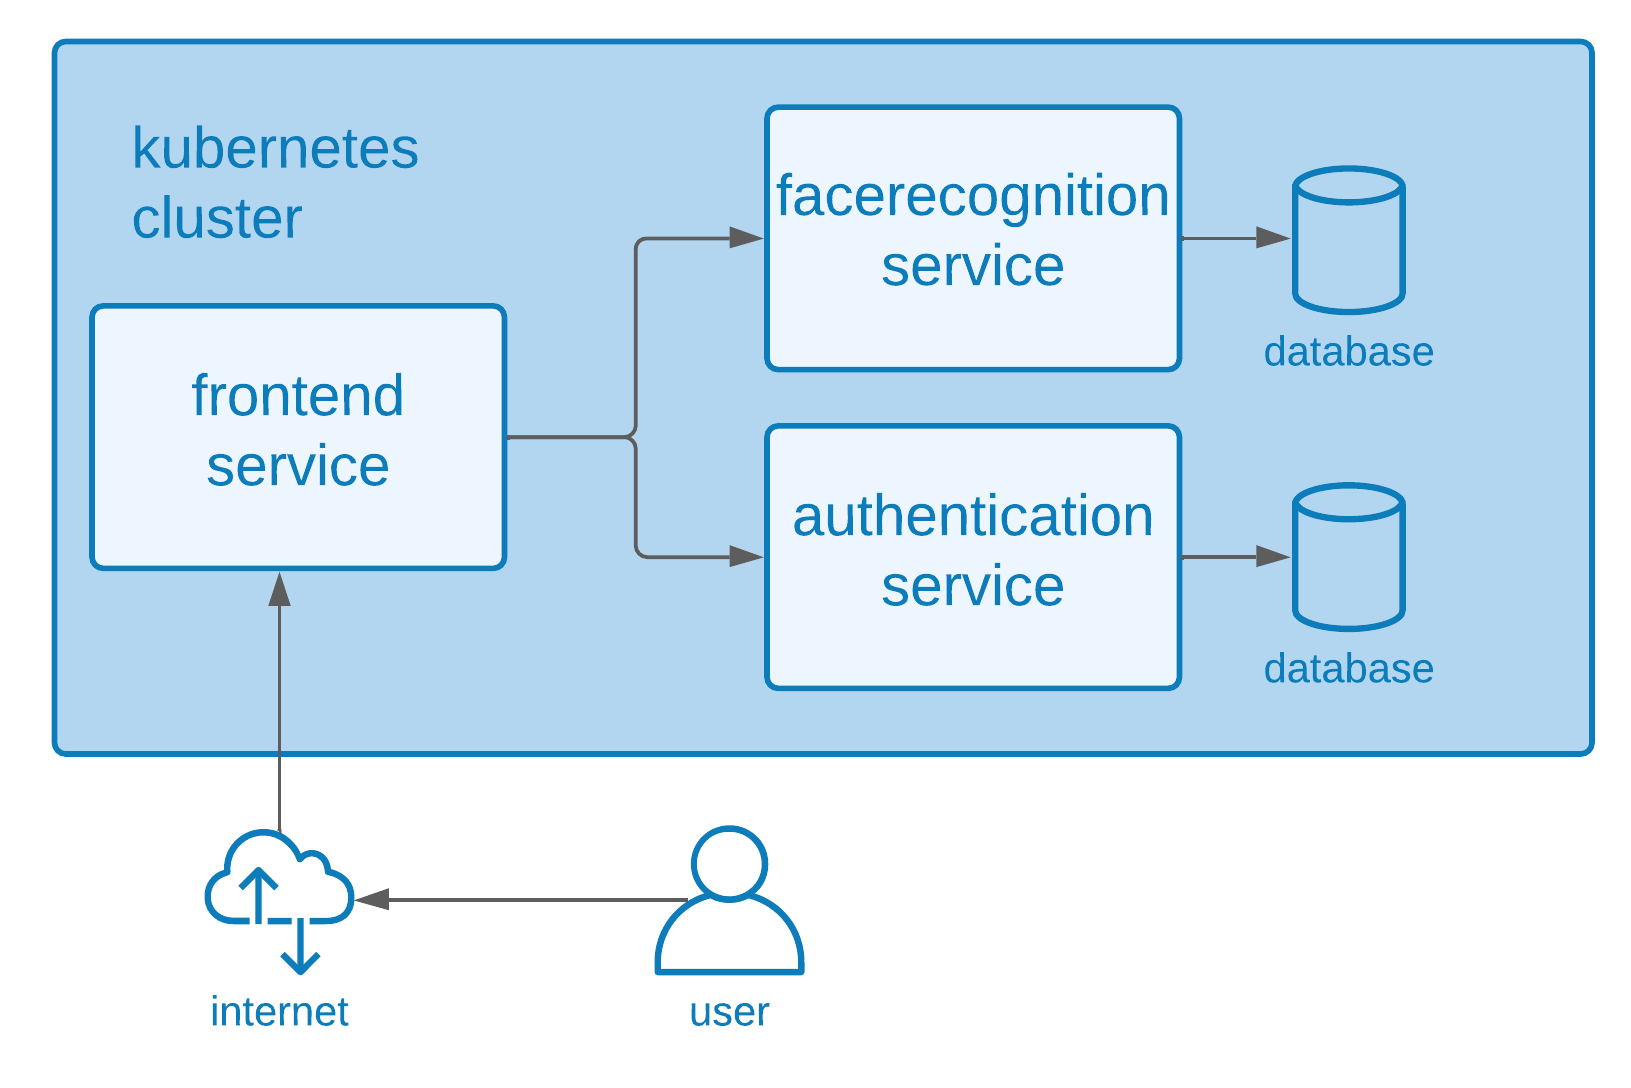
\includegraphics[width=0.8\columnwidth]{images/GrobentwurfAnwendung.png}
    \caption{Grobentwurf der Awendung}
    \label{fig:GrobentwurfAnwendung}
  \end{figure}

Die Abbildung \ref{fig:GrobentwurfAnwendung} stellt das Anwendungszenario aus dem Unterabschnitt \ref{Anwendungsszenario} dar.
Die Anwendung aus dem Szenario wird in drei Diensten aufgeteilt.

\textbf{Frontend-Service}: Das Dashboard wird über den Frontend-Service bereitgestellt.
Darüber kann ein Benutzer die Funktionalitäten anderer Dienste nutzen.

\textbf{Authentication-Service}: Die Anmeldung und Registrierung in ein Nutzerkonto erfolgt über den Authentication-Service.
Dieser ermöglicht die persistente Speicherung der Nutzerdaten.

\textbf{Facedetection-Service}: Der Facedetection-Service bietet eine Anmeldung mithilfe von Gesichtserkennung an.
Die relevanten Daten zur Gesichtserkennung werden in einer Datenbank persistent gespeichert.

\subsection{Mögliches Vorgehen}

Die Entwicklung der Anwendung wird in drei auf sich aufbauende Schichten eingeteilt.

\begin{figure}[!htb]
    \centering
    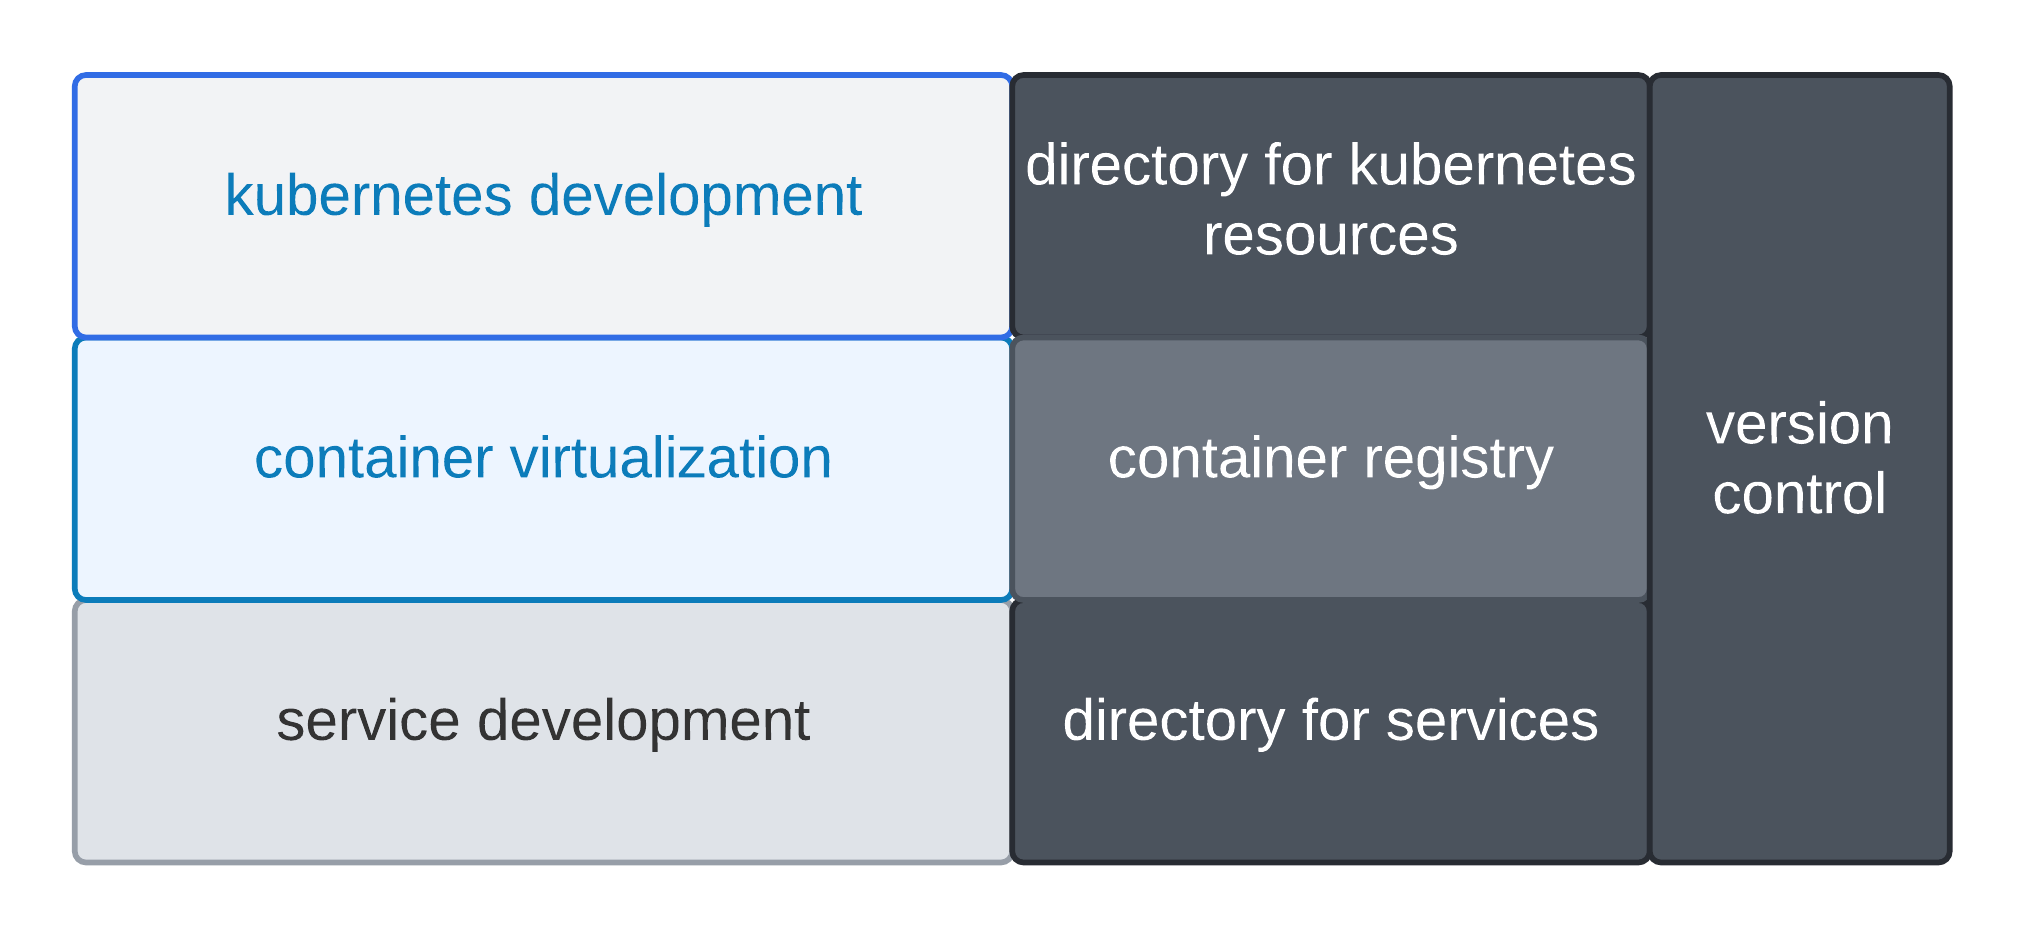
\includegraphics[width=1.0\columnwidth]{images/Schichtenentwurf.png}
    \caption{Vorgehen des Entwicklungsprozesses in Schichten}
    \label{fig:Schichtenentwurf}
  \end{figure}

\subsubsection{Anwendungsentwicklung}
Die Anwendung wird Anfangs erst für die Ausführung am lokalen Rechner entwickelt.

Einzelne Verzeichnise 

\textbf{Containervirtualisierung}: 
Das entwickelte Programm wird dann containerisiert und lokal ausgeführt.
Es wird getestet, ob die Containerisierung funktioniert und eine Kommmunikation
untereinander möglich ist. Schließlich wird das Image auf ein öffentliches Registry geladen.

\textbf{Kubernetes Deployment}: 
Das Testcluster wird aufgesetzt, installiert und in einen Rancher Server integriert.




